\documentclass[12pt]{ucthesis} \newif\ifpdf \ifx\pdfoutput\undefined
    \pdffalse % we are not running PDFLaTeX
\else \pdfoutput=1 % we are running PDFLaTeX \pdftrue \fi
\usepackage{url}
\ifpdf
    \usepackage[pdftex]{graphicx}
    % Update title and author below...
    \usepackage[pdftex,plainpages=false,breaklinks=true,colorlinks=true,urlcolor=blue,citecolor=blue,%
                                       linkcolor=blue,bookmarks=true,bookmarksopen=true,%
                                       bookmarksopenlevel=3,pdfstartview=FitV,
                                       pdfauthor={__author__},
                                       pdftitle={___Your_title_here___},
                                       pdfkeywords={thesis, masters} ]{hyperref}
    % Options with pdfstartview are FitV, FitB and FitH
    \pdfcompresslevel=1
\else
    \usepackage{graphicx}
\fi

\usepackage{longtable}
\usepackage{float}
\usepackage{amssymb}
\usepackage{amsmath}        % need for equations
\usepackage[letterpaper]{geometry} \usepackage[overload]{textcase}
\usepackage{graphicx}        % standard LaTeX graphics tool \usepackage{subfig} 
        % when including figure files

\newcommand{\thickhline}{\noalign{\hrule height 1.0pt}}
\newcommand{\tab}{$\hspace{6pt}$}
\newcommand{\mathbi}[1]{\textbf{\em #1}}
% %%%%%%%%%%%%%%%%%%%%%%%%%%%%%%%%%%%%%%%%%%%%%%%%%%%%%%%%%%%%%%%%%%%%%%%%%%%%%


\bibliographystyle{abbrv}

\setlength{\parindent}{0.25in} \setlength{\parskip}{6pt}

\geometry{verbose,nohead,tmargin=1.25in,bmargin=1in,lmargin=1.5in,rmargin=1.3in}

\setcounter{tocdepth}{2}

% Different font in captions (single-spaced, bold) ------------
\newcommand{\captionfonts}{\small\bf\ssp}

\makeatletter  % Allow the use of @ in command names
\long\def\@makecaption#1#2{%
  \vskip\abovecaptionskip
  \sbox\@tempboxa{{\captionfonts #1: #2}}%
  \ifdim \wd\@tempboxa >\hsize
    {\captionfonts #1: #2\par}
  \else
    \hbox to\hsize{\hfil\box\@tempboxa\hfil}%
  \fi
  \vskip\belowcaptionskip}
\makeatother   % Cancel the effect of \makeatletter
% ---------------------------------------

\begin{document}

\title{Smarter NEAT Nets}

\author{Ryan De Haven}
\degreemonth{December} \degreeyear{2013} \degree{Master of Science}
\defensemonth{October} \defenseyear{2013}
\numberofmembers{3} \chair{Franz J. Kurfess} \othermemberA{John Seng}
\othermemberB{Foaad Khosmood}
\field{Computer Science} \campus{San Luis Obispo}
\copyrightyears{thirteen}


\maketitle

\begin{frontmatter}

% Custom made for Cal Poly (by Mark Barry).
\copyrightpage

% Custom made for Cal Poly (by Mark Barry).
\approvalpage

 
\begin{abstract}
This paper discusses a modification to improve usability and functionality of a
genetic neural net algorithm called NEAT. The modification aims to accomplish
its goal by automatically changing parameters used by the algorithm with little
input from a user. The advantage of the modification is to reduce the guesswork
needed to setup a successful experiment with NEAT that produces a usable
Artificial intelligence (AI).

The modified algorithm is tested against the unmodified NEAT with several
different setups and the results are discussed. The algorithm shows strengths in
some areas but can increase the runtime of NEAT due to the addition of parameters into the
solution search space.

\end{abstract}

\begin{acknowledgements}

\end{acknowledgements}

\addcontentsline{toc}{chapter}{Contents}
\tableofcontents

\listoftables

\listoffigures

\end{frontmatter}

\pagestyle{plain}

\renewcommand{\baselinestretch}{1.66}


\chapter{Introduction}

Artificial intelligence (AI) is used in all video games in todays world, but
rarely are there games with AI that learns. By using machine learning in video
games or other AI applications, AI agents could improve as they compete against
users.
AI using machine learning or in the case of this paper, genetic algorithms, could
create an AI better than any programmer and could do so with little input from a
programmer. These genetic algorithms perform well on problems that require
searching for a solution that is arrived at by finding the best set of values
across a large number of variables.

Machine learning, specifically neural networks, has been used in games recently
such as Black & White 2 and the NEAT specific NERO \cite{hastings2009evolving}.
By using machine learning like neural nets programmers can create AI that
changes to adapt to the user or even generate content. This paper aims to
improve using the NEAT algorithm to allow machine learning to be easier and
better to use. 
 

\chapter{Background or Related Works}


\section{Genetic Algorithms}

Genetic algorithms (GAs) are a system that builds up solutions to a problem
space. GAs use a population of individuals that represent a solution to a given
problem. These individuals consist of genomes, descriptions of different parts
to a solution very much like genetic data (DNA) in biology. Over many
generations, GAs weed out bad solutions by only keeping genes from a top percent
of the individuals. Most GAs use a method called crossover to mate two parent
genomes selecting random genes and creating an offspring.As in biology, a key
feature of genetic algorithms is the mutation of genes across individuals. 
Mutation allows individuals to search for a solution by randomly changing parts
of the genome. GAs repeat the process of creating offspring until a solution of
acceptable quality is found.

Genetic algorithms show promise in the field of video games with research on
genetic AI \cite{Revello,PengHuo,Chih-Sheng}. Ever since the beginning of
genetic research with John H. Holland, applications of genetic algorithms have
been expanding. The new application of GAs in Neural network topology is
presented in the algorithms of SANE \cite{moriarty:focus} , ESP
\cite{gomez:proposal} , and GNARL \cite{Angeline}.


\section{Galactic Arms Race}

The Galactic Arms Race or GAR incorporates a type of NEAT for generating content
in the game called cgNEAT \cite{hastings2009evolving}. In this game the player
assumes the role of someone fighting aliens and using randomly generated
weapons.
The genetic algorithm cgNEAT generates the weapons for the player based
upon which weapons players in the game are collecting and using. The
neural networks created are compositional pattern producing networks that
generate the way the weapons looks\cite{hastings2009evolving}. Examples can be
seen in Figure Figure ~\ref{fig:weapons}.

\begin{figure}[h!] 
\caption{Different weapons created by cgNEAT}
  \centering
    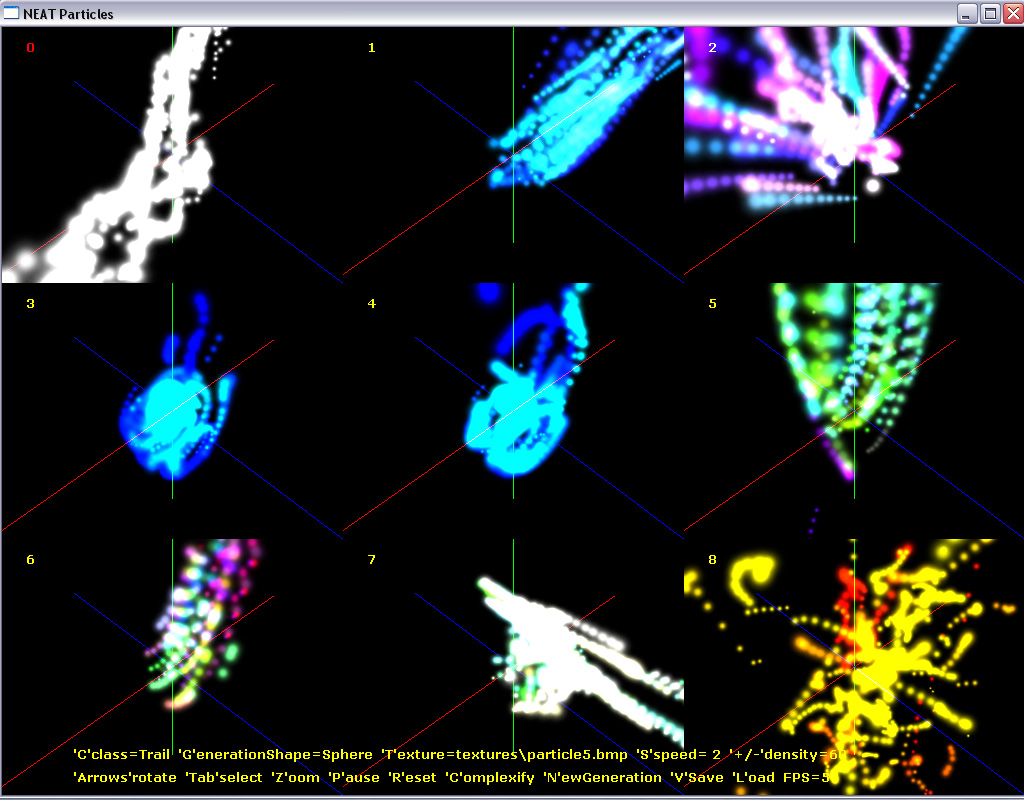
\includegraphics[width=0.5\textwidth]{weapons.jpg}
   \label{fig:weapons} 
\end{figure}

GAR starts the users in the game with a set of starter weapons that are preset
by the developers. Then players can find weapons spawned in the game world that
are created by cgNEAT. Items that are picked up by players and used are then
added to the population of offspring that will reproduce. An example of a weapon
evolving the game of GAR is shown in Figure ~\ref{fig:evoguns}.

\begin{figure}[h!] 
\caption{Evolution of weapons using cgNEAT}
  \centering
    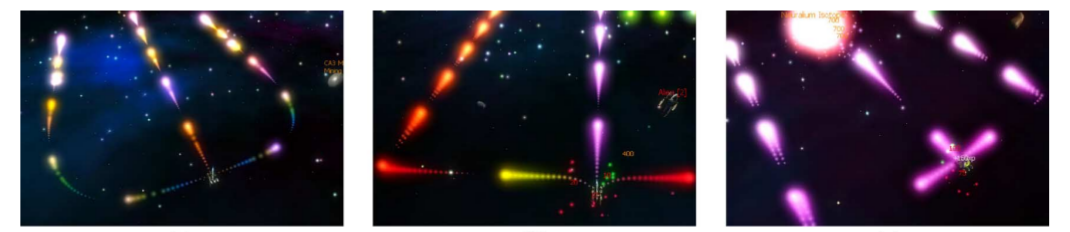
\includegraphics[width=0.9\textwidth]{evoguns.png}
   \label{fig:evoguns} 
\end{figure}

Due to players picking weapons that work better for them,
later generations perform better than earlier generations as seen in
Figure ~\ref{fig:evoguns}. GAR shows promising development for genetic algorithms that can create usable
content.

\section{Neural Genetic Agents: NERO}
  
Neuro-Evolving Robotic Operatives or NERO for short, is a game based on the
rtNEAT implementation of NEAT\cite{stanley:cig05}. In the NERO game the player
trains and uses robot units to complete certain tasks. The main part of the game play is
defending and capturing towers against another team of trained robots.

The most interesting aspect of NERO and rtNEAT is that the agents are created in
real time. This means that during training or gameplay agents will be removed
and replaced with new neural nets derived from the species in the given
population.
rtNEAT only selects parents for new agents from those that are old enough to
have been evaluated. This avoids the problem of removing the fit from the
population due to improper evaluation.

Training mode in NERO involves giving the player 50 units to run through a
course defined by the player. The player sets a spawn point for the robots where
they will have to move from and complete a certain task. After a set amount of
time the robots will be restarted from the spawn point with a new brain. The
restart is to make sure that no robot is at an advantage when it has its brain
replaced. As with the original NEAT neural nets for the initial robots start
with a randomly connected topology. The outputs and inputs default to a simple
approach with only 3 outputs and 13 inputs as shown in Figure ~\ref{fig:topology}.

\begin{figure}[h!] 
\caption{Inputs and outputs for NERO}
  \centering
    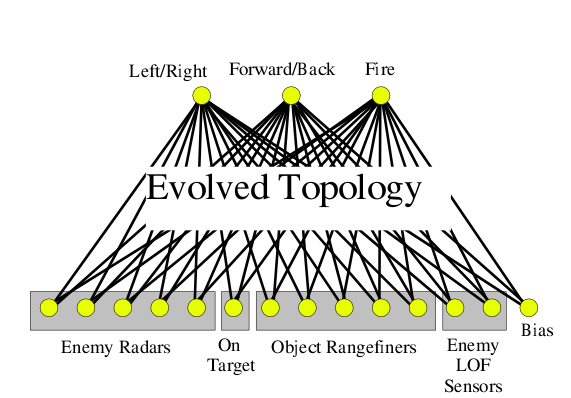
\includegraphics[width=0.5\textwidth]{topology.png}
   \label{fig:topology} 
\end{figure}

Players could set up different scenarios using obstacles such as turrets and
walls. The player would then give the robots a fitness score based on certain
performances of the robot. By training agents to do different tasks a player
could assemble a team of robots to face against another team. An example of of
training is shown in Figure ~\ref{fig:topology}.

\begin{figure}[h!] 
\caption{Robots navigating a maze}
  \centering
    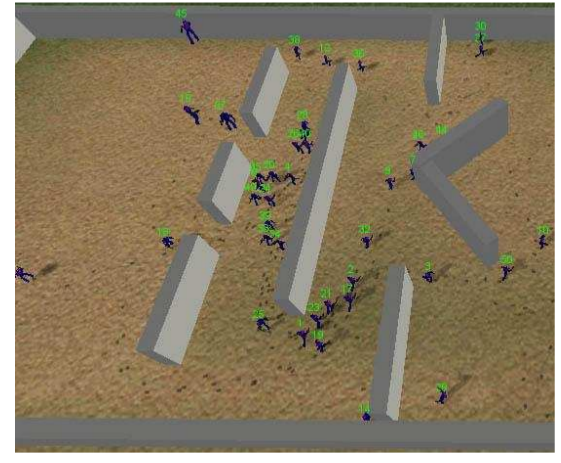
\includegraphics[width=0.5\textwidth]{robot.png}
   \label{fig:robot} 
\end{figure}

By allowing real time replacement the user can see clearly how the training is
affecting the algorithm and is improving the intelligence of the agents. For
this reason, NERO is a great way to learn about genetic algorithms and neural
net evolution.
 
\section{Artificial Neural Networks}

Neural networks aim to simulate the way the brain works by connecting neurons
as nodes to each other using links. In a brain the cells perform some operation on
the incoming signals and then send out signals to other neurons.
Neural networks have shown themselves to be useful for memorizing patterns and
solving parallel logic. Neural nets have shown promise in image recognition from
the beginning of its research \cite{lippmann}. Studies on animals have shown
that fully connected neural networks are what helps cats’ eyes recognized shapes
\cite{hubel1959receptive}.
Neural networks are made up of layers of nodes that feed into each other.
Usually the input nodes are the first layer that feed to the next layer and so
on until the output nodes are reached. Input and Output nodes are connected to
the program that is running the network and are ultimately what runs the AI.
There are different types of neural networks depending on the connections within
them. Neural networks with links from nodes either at the same level or towards
the input level are called recurrent networks. There are standard forms of
connected neural nets where all nodes are fully connected between each level of
nodes. NEAT does not follow this nor any other standard set of topology form,
due to its ability to generate topology randomly. Connections in nonstandard
graphs can connect from any level to any other level as long as they do not
travel towards the input nodes, if they do they are nonstandard recurrent
networks.
The operation each node performs is a sum across all of its input nodes and an
activation function using threshold logic, a binary function (on or off) or
sigmoid function. In NEAT the nodes activation function is always a sigmoid
function.

NEAT uses standard fitness sharing to determine how many individuals are
created from each specie. Fitness sharing simply uses the fitness of the species
over the total fitness of all individuals times the current population number to
calculate the offspring for the specie.

While NEAT uses simple genetic methods, it uses a unique way of comparing
structures that allow it to perform efficient evolution of topologies and is the
reason why it was chosen to study.

\section{NEAT Background}

NEAT or NeuroEvolution of Augmenting Topologies  was originally developed in
2002 and since then has been used in multiple games and developed extensively
\cite{stanley:phd04}. NEAT is a combination of neural nets and genetic
algorithms to create an algorithm that build on a simple neural net and evolve it over many
generations. NEAT evolves both the connection and weights on nodes incrementally
improving the network. These type of algorithms are called Topology and Weight
Evolving Artificial Neural Networks or TWEANNs. NEAT solves the problem of
protecting newly created structures in its genome through speciation. This way
topologies can be formed in their own specie and evolve without directly
competing with other individuals outside their own specie. Most TWEANN’s do not
use speciation due to the problem of fitting individuals into distinct species
since grouping similar topologies is difficult. NEAT solves this problem by
recording historical information about each new gene. Each new gene that is
added is given a global innovation number. Each topological change can then be
tracked by this number. Individuals are grouped into species by comparing each
individuals connection and node genes. The comparison checks for genes that have
the same innovation number in both genomes, the genes that do not match are
called excess or disjoint genes. Excess genes are genes that fall beyond the
innovation number of the last gene in the first genome being compared. Disjoint
genes are merely the genes that do not match innovation numbers, but they
numbered at or before the last innovation number in the first parent being
compared. An example can be seen in  Figure ~\ref{fig:parentgenes}. In order to fit
individual members into species, each member is compared with a previous
representative for each past specie. These representatives are chosen at random
from the past generation. The individual is placed into the first specie
possible if the calculated value of $\frac{c_{1}E}{N} + \frac{c_{2}D}{N} + c_{3}
\cdot \overline{W}$ falls below a certain threshold parameter $\delta$ , where E are
the number of excess genes, D is the number of disjoint genes, and N is the
number of genes in the larger genome. Constants $c_{1} - c_{3}$ determine how
much each variable affects the comparison. If there is no match when comparing all of the previous species then a new specie is created and the individual is added to that specie.

\begin{figure}[h!] 
\caption{The production of offspring and gene characteristics
\cite{stanley:phd04}}
  \centering
    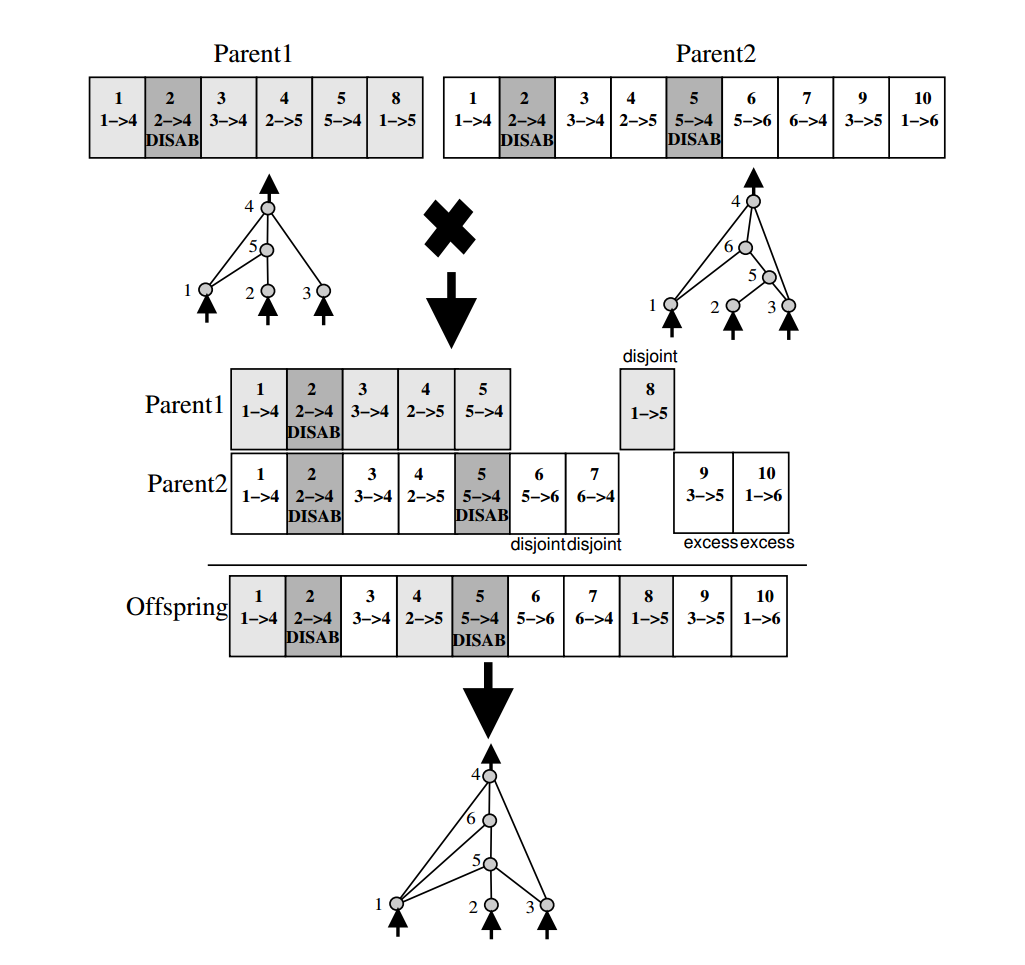
\includegraphics[width=1\textwidth]{parentgenes.png}
   \label{fig:parentgenes}
\end{figure}


\section{Mario Platform}
Mario from the famous Nintendo game, Super Mario Bros. The platform
that is used in this paper is called Mario AI benchmark and has been used in
numerous competitions \cite{karakovskiy2012mario}. The platform was chosen as a
testbed due to ease of benchmarking and comparing results on a well
known game. The platform allows for randomly generated levels, allowing for
variety of difficulty. The difficulty can range from a flat level with no pits to large
pits with many obstacles. The Mario AI benchmark supplies an API that makes it
easy to interact using an AI. The API can supply the AI positions of enemies, blocks, and states
that the Mario sprite is in. The grid layout that represents the Mario sprites
vision is shown in Figure ~\ref{fig:mariogrid}. The agent interface supplies a method
that outputs Mario’s buttons presses for each 40ms frame. The allowed buttons
are A (jump) , B (run / grab shell) , and the directionals: left, right, up,
and down. The benchmark records scores on distance traveled, kills, and items
collected so these scores can be used in heuristics and benchmarking.

\section{Tetris Platform}

Tetris is one of the must successful and widely known games. It was created by
Alexet Panitnov in 1984 in the Soviet Union. The gameplay of Tetris is a puzzle
game where the player must fit different shaped pieces to form lines of blocks.
These blocks are then removed that the above blocks slide down. Game pieces are
allowed to by rotated into 4 different rotations and move left and right.
Application of Tetris in this paper use a Tetris clone developed by professors
at Stanford for teaching students about AI \cite{tetris}. This
platform was chosen due to the easy API developed for creating an AI to work with Tetris. The coding platform
lets the user define a generic size Tetris board represented by a grid of boolean
values. The value of each cell in a grid shows if there is a Tetris block place
there or not.

\begin{figure}[h!] 
\caption{The mario vison grid}
  \centering
    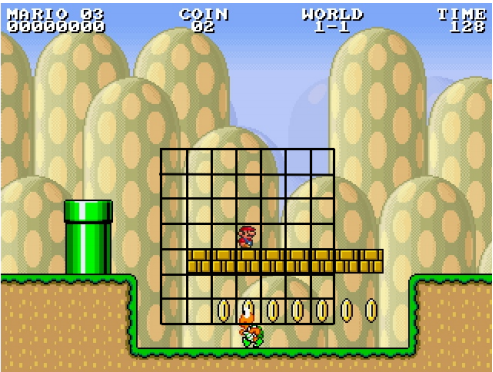
\includegraphics[width=0.5\textwidth]{mariogrid.png}
   \label{fig:mariogrid} 
\end{figure}

\chapter{Algorithm}

In order to asses the difficulty of creating an AI interface for use in the NEAT
environment, a Tetris game was reworked with NEAT and the difficulties were
recorded. The Tetris game that was used came from a beginning programing class
and had an interface for AI that most games would have before implementing any
kind of neural nets \cite{tetris}. Before starting to code the interface between
the Tetris AI and the genetic neural algorithm a few hypothesis were made:

\begin{itemize}
\renewcommand{\labelitemi}{$\bullet$}
\item Writing the interface / test harness interface would be simple (only take one
try) 
\item Tetris would perform well compared to normal AI provided
\end{itemize}

Tetris only took a few hours to code into the testing harness that was already
implemented. The most difficult part was changing the Tetris AI interface to
accept suitable neural inputs and return some kind of vision to the AI. The AI
originally was given a board state then asked for the best move given a piece
and a next piece. The move was a position (x,y) and a rotation of the given
piece. This was changed to better suit the neural net, giving it boolean inputs
for the board and what the piece looked like. Instead of asking for a move for
each piece the AI was asked for a move each cycle of the game, more like what a
human would experience while playing. After making these changes, the Tetris AI
was tested with the NEAT harness and was able to control the game.

After testing Tetris with the initial inputs and outputs as the whole board, it
became apparent that the AI was having trouble figuring out that it should be
trying to place pieces to score lines. The AI would at best put pieces to the
left then the right. This was due to the setup and shortsightedness of the
programmer. Since the neural net had inputs for the whole board (10 by 20
blocks), it was receiving over 200 inputs, much higher than that of the AI mario
tests (around 50). In order to achieve a correct move, the neural net would have
to memorize exact board states. With 200 inputs the genetic NEAT algorithm would
have to randomly create weights for the connecting inputs. After 10 runs, the AI
never scored higher than 1 line.

The next implementation used a more roaming eye approach as described in
\cite{stanley:phd04}. This approach helps simplify the amount of inputs by
giving the AI a small moving subset of vision instead of the whole board. After
implementing the modifications to the original AI a series of tests were run to
see if there was improvement. Again, the AI failed to gain more than one line.

In order to debug the program to find the reason for failure, I printed out the
grid of vision each time the AI was run. I found a small error with converting a
grid of booleans to the neural inputs. After fixing the error, the AI still
behaved poorly. For further testing, the Tetris pieces the AI was given during testing
was set to only vertical bars. While observing the AI, I found it having trouble
with the edges of the Tetris board. Vision outside of the tetris board had been
set to empty in the AI code, giving the AI the appearance of a place to put the
piece after it had discovered how to place lines. This problem was easily solved
by filling the outside of the game area with filled in blocks (as if there were
Tetris pieces filling it in).

\section{NEAT Interface}

The genetic description about how to initialize the neural network and how to
genetically change the individuals is loaded from a .ga file at startup. The
file contains parameters for settings such as the genetic crossover rates and
mutation rates. In order to simplify the testing process a GUI was created to
automate the experiments, allow easily changing parameters, and observe
collected data across runs.

The created interface simplifies the testing process of NEAT and allows the user
to change datasets (Mario levels) mid run and observe changes in species and
individuals through lists of data. Demos can be run of any individual or
individual with the best fitness for that generation. These demos show the
neural net structure described by the genome and run the AI on the selected task of
Tetris or Mario. The visualization code was supplied by the NEAT4j code base
and an example can be seen in Figure ~\ref{fig:simplemarionet}.
These demos are threaded so they can be run while still performing the
experiment.

Each specie present in the current experiment is displayed in a list showing the
number of individuals in each specie. Selecting a specie shows the
individuals in that specie.
Selecting an individual shows each gene present in the genome and selected
information for each gene. If a self-regulation gene is present in the genome
then the contents of that gene are shown in a separate box. These information
boxes are useful for debugging, especially for debugging the self regulation
gene's affect on the algorithm.

Both the Tetris and Mario mode of the interface are threaded to decrease the
runtime of long experiments. Only the testing phase of the genetic algorithm is
multi-threaded as this is where most of the runtime is located.

For the Mario testing there is a level queue that allows setting up any number
of levels at any difficulty.  Marios vision parameters can be changed as well as
all the parameters as described in the NEAT4j section. Each run can be set to
automatically restart at a set breakpoint of a number of generation or a maximum
score reached.

There is a graphing tab in the GUI interface that allows for viewing the total
fitness of the population over a history of runs. The graph tool is useful for
debugging changes to the NEAT algorithm as well as the AI interface between the
neural net and the game it is controlling. For example, while creating the AI
interface between Tetris and the neural net there was a clear improvement when
allowing the neural net to use the level of the current Tetris block as an
input. 

\begin{figure}[h!]
  \caption{An example of a neural network demo}
  \centering
    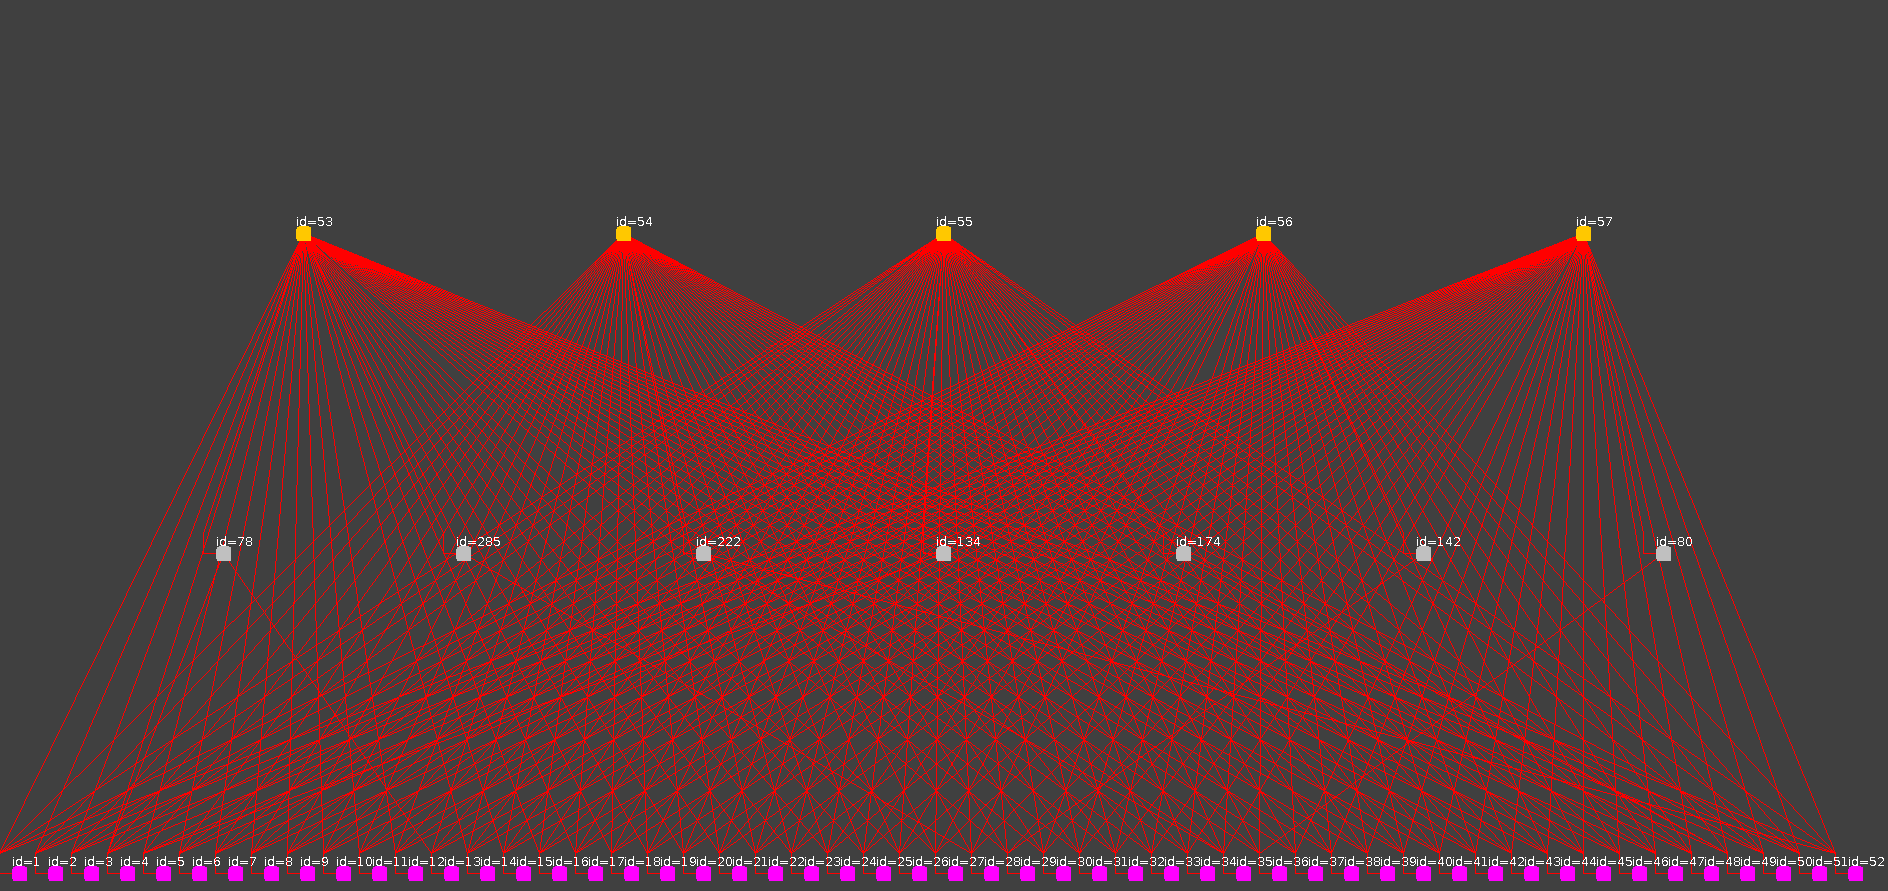
\includegraphics[width=1\textwidth]{simplemarionet.png}
   \label{fig:simplemarionet} 
\end{figure}


\chapter{Algorithm: Experiments with NEAT and Mario}


In this section the process of implementing a system that allows the
application of NEAT to a general set of AI problems will be discussed. The
software that was modified for this was the NEAT4J implementation of NEAT
written in Java. The NEAT algorithm was selected due to its success in NERO and
other games.

Heuristics that help promote a correct solution are critically important for
GA’s to work correctly. Finding heuristics that work appropriately for GA’s can be
tedious or impossible to find if the search space for the neural network is too
large.
In order to solve the aforementioned problems, the first experiment was to allow
for each genome run to determine its own heuristics. A new genotype was added
called a self regulation gene. This gene contains numerical values for the
heuristics in the Mario game. The default heuristics that were used are shown in
~\ref{tab:Heuristics}. Although for the Mario game the number of different
heuristics was short, the number could be much greater in more complex games.
While experimenting with NEAT, the amount of set up and tweaking of variables seemed to be too much of a hassle
for a normal user.  I tried a couple of modifications to the NEAT algorithm to
alleviate the difficulty of using NEAT.  These modifications added a new gene that determined specific heuristic changes to be used during the speciation
process where only the individuals with the highest fitness are used to populate
the next generation.

Each specie would use its highest fitness individual’s self regulation gene to
determine the heuristics for all individuals that fit into the specie. The
reason behind this was to not allow an individual to just give themselves larger
and larger heuristic values. The self rating was called the self fitness value.
This value was then averaged with a baseline default heuristic value to further
prevent self heuristic inflation. The results are shown later in Chapter
~\ref{chp:Results}.

The first algorithm explored gave each individual in generation 0 a random
heuristic values so each gene would be a unique set of heuristic values. This
would work well for small sets of heuristic values to search through or
situations where changing the heuristics mid-run will ruin the population. If the ability
for heuristics to change dynamically was added then the GA would be able to
change as needed to improve the overall fitness while adjusting specific
heuristics within each specie. This was the hypothesis that led to another
change that would let the self regulation gene guide the whole genetic algorithm
while changing parameters for NEAT dynamically. These parameters that would be
changed are listed in Table ~\ref{tab:Parameters}. As well as containing these
parameters, the self regulation gene would contain additional parameters for
mutating all parameters in the self regulation gene.
For example, the pMutatateRegulationHeuristics variable would change the
probability that a heuristic is changed by at most the variable
PerturbRegulation.


\section{Initial Agent Implementation}

Most of the implementation work involved creating the framework to allow NEAT to
control Mario agents in Infinite Mario. I used the NEATGATrainingManager class
in NEAT4J as a starting place to create and evaluate agents.
After figuring out how to run experiments I created an agent for
Infinite Mario that took in a neural net from NEAT and connected the appropriate
inputs and outputs. Once Mario started jumping around with a default configuration I moved
to tweaking the program to get a Mario that could complete static levels.
In order to make sure the algorithm was creating good Mario agents I set up a
system that allowed the user to see each agent's fitness score at the end of its
test and every time a Mario completed a level it would display that Mario net
actually doing the level. NEAT also let me visualize the neural net topologies
that were being generated. That way I could see how each setting changed how the
neural nets were formed. Eventually, the heuristic values shown in Table
~\ref{tab:Heuristics} were found to result in well performing Mario AIs.
 
\begin{longtable}{| l | c |}
  \hline
  Heuristic & Default Value \\ \hline                   
  Distance travelled & 1  \\ \hline
  Mushrooms collected & 0 \\ \hline
  Flowers collected & 0  \\ \hline
  Coins collected & 0  \\ \hline
  Stomp kills & 200  \\ \hline
  Shell kills  & 500  \\ \hline
  Connection genes  & 0  \\ \hline
  Total Nodes  & 0  \\ \hline

\caption{Table of default heuristics for the Mario genetic
 algorithm}
\label{tab:Heuristics} 
\end{longtable}

\chapter{Results}
\label{chp:Results}

The goal of this experiment was to create a modification to the neat algorithm
that would automatically vary parameters for NEAT rather spending hours
tweaking settings files. The results show improvements in some areas, however
this method has some pitfalls and shortcomings as revealed by experiments.

All tests using the Mario testbed were implemented by giving a vision grid with
one block behind Mario and 5 blocks ahead of Mario, 3 blocks above Mario and 5
blocks below Mario. Other inputs include a bias input of 0, an input if Mario is
carrying a shell, an input that determined if Mario can jump and an input if
Mario is on the ground. These inputs totaled to 52 inputs with 5 outputs for each button Mario
could press. Mario was also given the ability to jump by continuously holding
the jump button down, making the logic more simple to evolve.

\section{Results for Mario Running NEAT with the Same Heurisitics}
The Mario benchmark was run with various setting for NEAT4j and a population
size of 500. All heuristic values were set to 1 across these experiments. As
a base for comparison a run with the default parameters values as listed in
Table ~\ref{tab:Parameters} is presented. For the base run the total fitness graph
Figure ~\ref{fig:defaultave} shows a problem keeping fitness as the number of species
changes. This is due to the compatibility threshold fluctuating to compensate
for the number of species which started at 500, the same as the population
number. The algorithm is trying to keep the number of species to 15 by
changing the $\theta$ value as seen in Figure ~\ref{fig:defaultspecies}. As this value
changes genes can be lost as species combine with others, which is why a
fluctuation in average fitness is observed.

In comparison to using a limited feature set of the self regulation gene and
compatibility change enabled, the default parameters configuration converged to
a solution in about 10 generations while the self regulation implementation takes 50 to 80
generations as seen in Figure ~\ref{fig:defaultbest} and 
Figure ~\ref{fig:selfreg_default_best}. This is due to the starting parameters of the
self regulation genes starting at much smaller mutation rates than the default
parameters. The self regulation gene is set this way to avoid creating species
that mutate too fast too early.
When the level difficulty is changed to a harder level the self regulation gene
helps increase mutation rates. As shown in 
Figure ~\ref{fig:selfreg_default_hard_best} and Figure ~\ref{fig:default_hard_best} the normal
NEAT algorithm has parameters set too low to develop any solutions to the
problems it is facing.

The best improvement is seen when all the parameters for the self regulation
genes are randomly chose as each gene is created. This allows for a larger
diversity of parameters and sometimes a faster convergence on a solution. graph
Figure ~\ref{fig:selfreg_random_hard_best} shows that seeding random values for self
regulation parameters helps improve the chance of finding a solution as compared
with self regulation without randomization. The graph also shows that using this
method will not always yield the same result, since run 1 and run 2 of the
algorithm in Figure ~\ref{fig:selfreg_random_hard_best} did not find the same solution.

The tests using the Mario platform revealed that the self regulation gene helped
in cases where the difficulty of finding a solution was higher than expected and
NEAT parameters needed to be adjusted to compensate. Otherwise, the self
regulation gene improved the overall fitness of the algorithm and slightly
decreased the best fitness.

\begin{figure}[h!]
  \caption{Average fitness using default parameters}
  \centering
    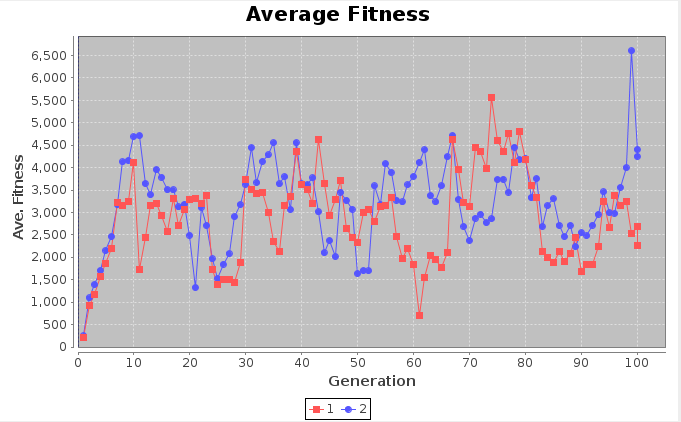
\includegraphics[width=1\textwidth]{graphsone/defaultave.png}
   \label{fig:defaultave} 
\end{figure}

\begin{figure}[h!]
  \caption{Number of species using default parameters}
  \centering
    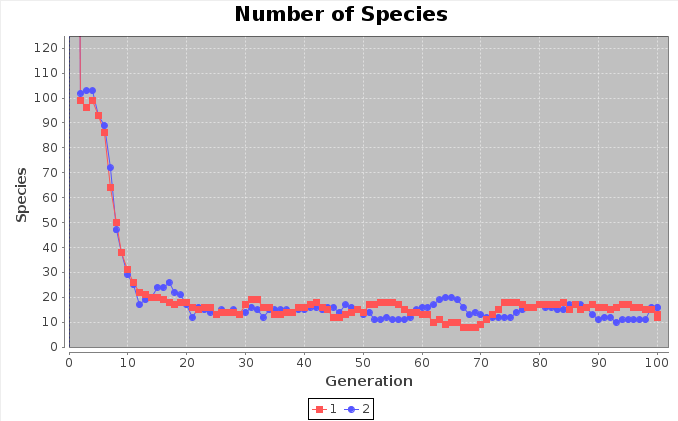
\includegraphics[width=1\textwidth]{graphsone/defaultspecies.png}
   \label{fig:defaultspecies} 
\end{figure}

\begin{figure}[h!]
  \caption{The best fit individual using default parameters}
  \centering
    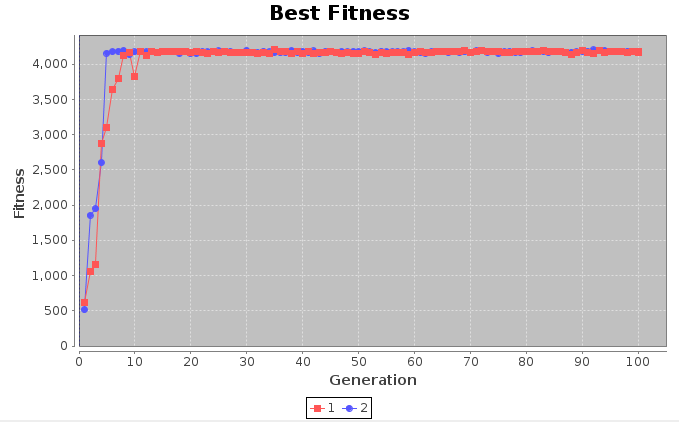
\includegraphics[width=1\textwidth]{graphsone/defaultbest.png}
   \label{fig:defaultbest} 
\end{figure}

\begin{figure}[h!]
  \caption{The best fit individual using self regulation gene}
  \centering
    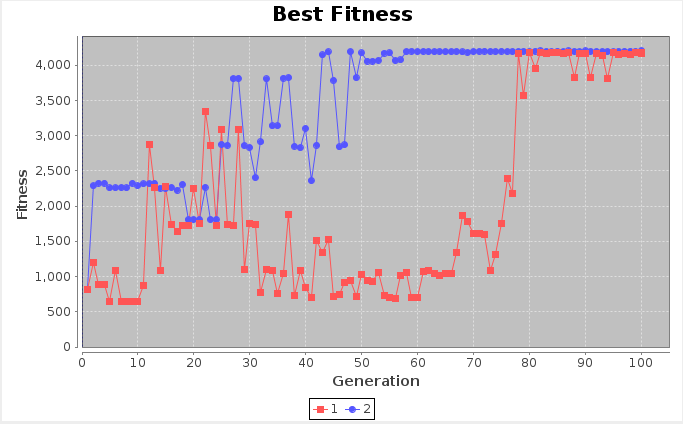
\includegraphics[width=1\textwidth]{graphsone/selfreg_default_best.png}
   \label{fig:selfreg_default_best} 
\end{figure}


\begin{figure}[h!]
  \caption{The best fit individual using self regulation gene on hard
  difficulty}
  \centering
    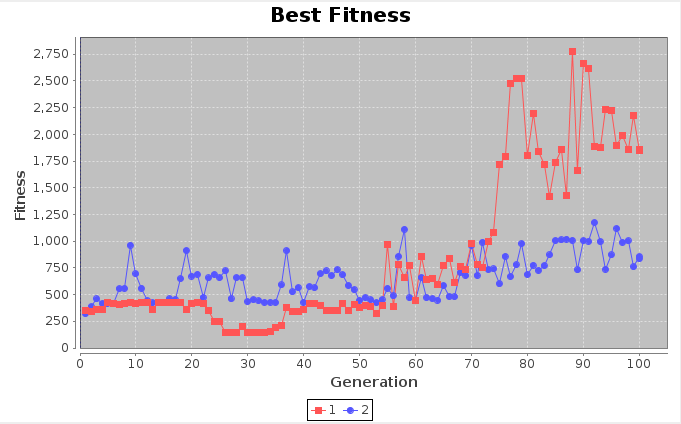
\includegraphics[width=1\textwidth]{graphsone/selfreg_default_hard_best.png}
   \label{fig:selfreg_default_hard_best} 
\end{figure}

\begin{figure}[h!]
  \caption{The best fit individual using default parameters on hard difficulty}
  \centering
    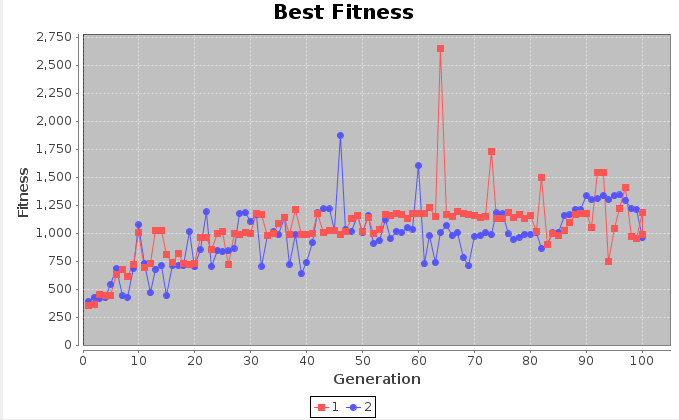
\includegraphics[width=1\textwidth]{graphsone/default_hard_best.png}
   \label{fig:default_hard_best} 
\end{figure}

\begin{figure}[h!]
  \caption{The best fit individual using self regulation gene with random
  parameters on hard difficulty}
  \centering
    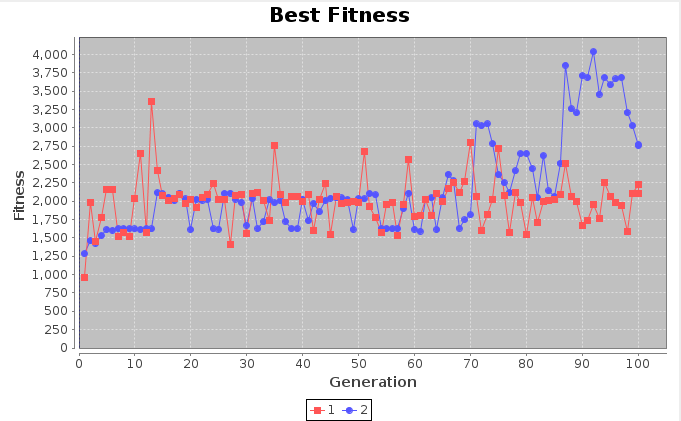
\includegraphics[width=1\textwidth]{graphsone/selfreg_random_best.png}
   \label{fig:selfreg_random_hard_best} 
\end{figure}


\section{Results for Tetris Running NEAT}
For these tests the Tetris environment has a board set to height of 6 by a width
of 10, since height is not a factor. For the heuristic values a line is given a
value of 10 and a piece placed is given a value of 1. There is a board rater
that rates a given board state and gives a value. The board raters score is
added for the last tick of the AI as the game ends. For each generation each
individual is run against three levels: one with a seed of 0, one with a seed of
2, and one with a random seed. The resulting fitness score is the sum of all the
levels.

The complexity of memorizing pieces and places to put the pieces seems to be
difficult for NEAT. All of the tests show that at best out a of a population of
500 there is at least one individual that scores a 90 as seen in
Figure ~\ref{fig:default_best_tetris} and Figure ~\ref{fig:self_best_tetris}. This is the 
equivalent to scoring 9 rows across 3 levels of Tetris. In previous test runs
NEAT was able to converge on solutions to levels with only line pieces showing
that the AI could solve simple problems.



\begin{figure}[h!]
  \caption{The best fit individual using default paramters for Tetris}
  \centering
    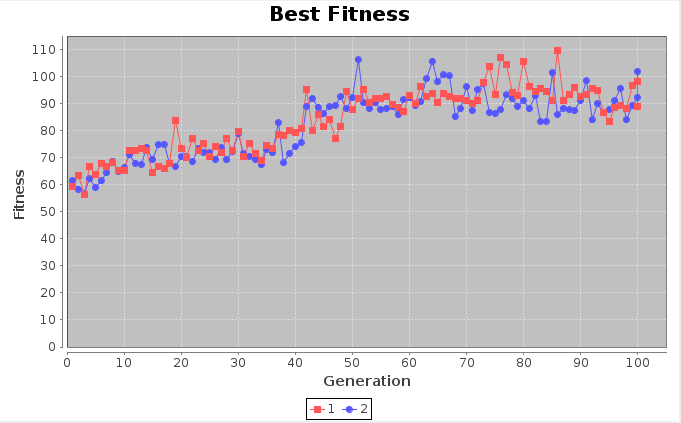
\includegraphics[width=1\textwidth]{graphstetris/default_best.png}
   \label{fig:default_best_tetris} 
\end{figure}
 
\begin{figure}[h!]
  \caption{The best fit individual using self regulation for Tetris}
  \centering
    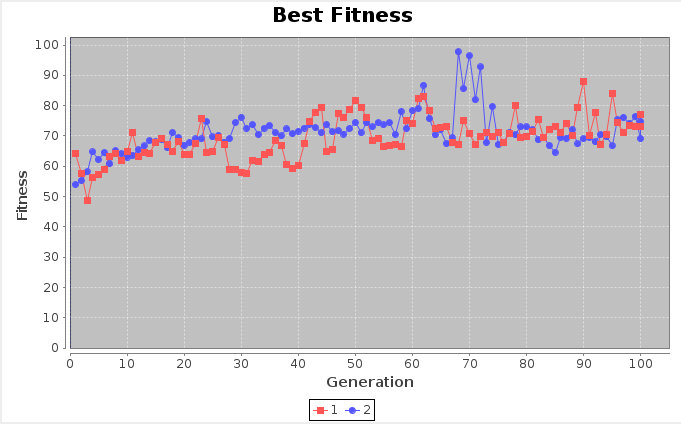
\includegraphics[width=1\textwidth]{graphstetris/self_reg_best.png}
   \label{fig:self_best_tetris} 
\end{figure}


\chapter{Conclusions and Future Works}
\section{Conclusions}
The self regulation gene has the potential to reduce the time needed to
configure an experiment with NEAT, as long as the experiment is difficult enough
that the normal parameters are not sufficient.

Defining useful heuristics is still important since there isn't a way to use the
self regulation gene to assign heuristic values used in calculating specie size.
As seen with the development of the Tetris interface, it is important to provide
inputs that work well with neural networks.

Overall the self regulation gene is an improvement to NEAT, but should only be
used in situations where a default setup is not providing results.

\section{Future Works}

\subsection{Different Genes}

An alternate approach to the implementation of the self regulation gene using
multiple genes containing information on specific parameters could lead to
improved convergence on parameters. This improvement would allow for genes to be
used only where they are needed, instead of using all the parameters present in
NEAT.
\subsection{Dynamic Data Set Selection}

In addition to generating heuristic values for the datasets or levels used to
run the AI against, datasets or level could be selected from a set to improve
AI creation. Selections could be made on  the difficulty the AI has solving certain
levels or levels that are shown to have a history of producing high fitness
individuals.
\subsection{Improved Specie Allocation}

There are a few parts of the NEAT algorithm that conflict with goals of the
modification. The distribution of individuals could be improved so that genes
are protected better during dynamic speciation. In some of the tests it was
apparent that too many species were being created and destroyed in order to keep
the number of species constant. This led to a large drop in the total fitness of
whole population. Either creating a modification to the dynamic compatibility
threshold algorithm or allowing the self regulation gene to have more control
over speciation could be explored to solve this issue.
\subsection{Aging}

Allowing the self regulation gene was tested in preliminary experiments and
showed problems due to species developing higher and higher youth boost
parameters. Species would inflate their own fitness without actually improving
anything. If this problem could be fixed then the aging functionality, allowing
modification of the specie age threshold, the specie youth threshold, the specie
old penalty , the specie age threshold, and the specie youth threshold could be
dynamically changed and solved.


\clearpage
\bibliography{references}
\bibliographystyle{plain}
 
\chapter{Appendix}

\begin{longtable}{| l | p{6cm} | c  | c |}
  \hline
  Parameter Name & Parameter Description & Range & Example  \\ \hline
  PROBABILITY.MUTATION & This value controls the mutation of connection weights
  and the sigmoid factor of the neurons. & 0 - 1  & 0.25 \\ \hline
  PROBABILITY.CROSSOVER & This value controls the rate at which individuals,
  within the same specie, perform a GA crossover operation as defined in the
  NEAT algorithm. & 0 - 1  & 0.2 \\ \hline PROBABILITY.ADDLINK & This is the
  rate at which new links are added between neurons. It does not take into
  account the recurrent parameter as this check is performed at the end of a
  mutation. & 0 - 1  & 0.05 \\ \hline PROBABILITY.ADDNODE & This is the rate at
  which new neuron is added to an enabled link. & 0 - 1  & 0.03 \\ \hline
  PROBABILITY.MUTATEBIAS & Each neuron has a bias value. This parameter controls
  the rate at which they are mutated. & 0 - 1  & 0.3 \\ \hline
  PROBABILITY.TOGGLELINK & A link (neuron-neuron connection) has two states,
  enabled and disabled. This paramter controls the rate at which a link might
  toggle its state. & 0 - 1  & 0.3 \\ \hline PROBABILITY.WEIGHT.REPLACED & A
  link can have its weight reset to some arbitrary value regardless of its
  current value. This parameter controls the rate at which this happens. & 0 - 1
   & 0.3 \\ \hline EXCESS.COEFFICIENT & A NEAT specific coefficient that
  provides a measure of importance to the excess of genes, within a chromosome,
  when it comes to calculating the compatibility between two chromosomes. &
  \textgreater=0 & 1 \\ \hline DISJOINT.COEFFICIENT & A NEAT specific
  coefficient that privides a measure of importance to the difference of genes,
  within a chromosome, when it comes to calculating the compatibility between
  two chromosomes. & \textgreater=0 & 1 \\ \hline 
  WEIGHT.COEFFICIENT & A NEAT
  specific coefficient that provides a measure of importance to the weight
  differences of link genes, within a chromosome, when it comes to calculating
  the compatibility between two chromosomes. & \textgreater=0 & 3 \\ \hline
  COMPATABILITY.THRESHOLD & A speciation parameter that is used when deciding if
  a given chromosome should go in a given species. & \textgreater=0 & 3 \\
  \hline COMPATABILITY.CHANGE & If this is 0, then the COMPATABILITY.THRESHOLD
  will not change at all. This means that the number of species will be not
  controlled.
  If this is greater than 0, then the COMPATABILITY.THRESHOLD will by
  dynamically changed (*up or down) by this change value to try and keep the
  number of species to be SPECIE.COUNT. & \textgreater=0 & .1 \\ \hline
  SPECIE.COUNT & A speciation parameter that is used when deciding if
  a given chromosome should go in a given species. & \textgreater=1 & 15 \\
  \hline
  SPECIE.COUNT & A speciation parameter that is used when deciding if
  a given chromosome should go in a given species. & \textgreater=1 & 15 \\
  \hline
   SURVIVAL.THRESHOLD & During mating within a species, this value defines the
   fraction of the top specie members that are allowed to mate. For example, if
   the value was 0.2, then only the fittest 20\% of the specie would be allowed
   to mate. & \textgreater=0 & .4 \\
  \hline
   SPECIE.AGE.THRESHOLD & Once a species age reaches this value, the fitness
   of the specie members will be multiplied by SPECIE.OLD.PENALTY. &
   \textgreater=1 & 80 \\
  \hline
    SPECIE.YOUTH.THRESHOLD & Whilst a species age is less than this value, the
    fitnesses of the specie members will be multiplied by SPECIE.YOUTH.BOOST &
   \textgreater=1 & 10 \\
  \hline
    SPECIE.OLD.PENALTY & The penalty applied to the fitness of a given species
    members. Note, if NATURAL.ORDER.STRATEGY is true, this should be \textgreater= 1 else
    \textless= 1 & \textgreater=1 or \textless= 1 & 1.2 \\
  \hline
  
  
\caption{Table of Parameters for NEAT4J}
\label{tab:Parameters} 
\end{longtable}

\end{document}reference.  